% Nome do capítulo
\chapter{O ambiente Node.Js}
% Label para referenciar
\label{ambiente-node-js}

% Diminuir espaçamento entre título e texto
\vspace{-1.9cm}


  Criado por Ryan Dhal em 2009, a plataforma Node.Js tem como objetivo mitigar o problema descrito no capítulo \ref{introducao}
  e prover um ambiente de programação amplo e forte para os desenvolvedores. 
  
  Nas próximas seções será explicado ao leitor as principais características do ecosistema do Node.Js.
 
  
\section{Programação Orientada a Eventos}
\label{programacao-orientada-a-eventos}

  A programação orientada a eventos é a principal abordagem para o sucesso do Node.Js. Sendo escolhida para
  minimizar os impactos de alta concorrência descrito anteriormente no capítulo \ref{introducao}. 
  
  As aplicações criadas com o Node.Js tem como núcleo e referência os eventos. Estes eventos são indicações de que ocorreu algo, 
  havendo dois atores para este modelo de programação.\cite{Oliveira:2012}
  \citeonline{Junior:2012} utiliza a terminologia de produtor do evento (\textit{event producer}) 
  e o consumidor do evento (\textit{event consumer}) para identificar estes dois atores. Em contrapartida os servidores
  web tradicionais utiliza o conceito de ação e resposta.
  
  
  \begin{figure}[H]
    % Alterar espaçamentos antes e depois do caption
    \setlength{\abovecaptionskip}{0pt}
    \setlength{\belowcaptionskip}{0pt}
    % Caption
    \caption[Ciclo de eventos no Node.Js]{Ciclo de eventos no Node.Js}
    \centering
    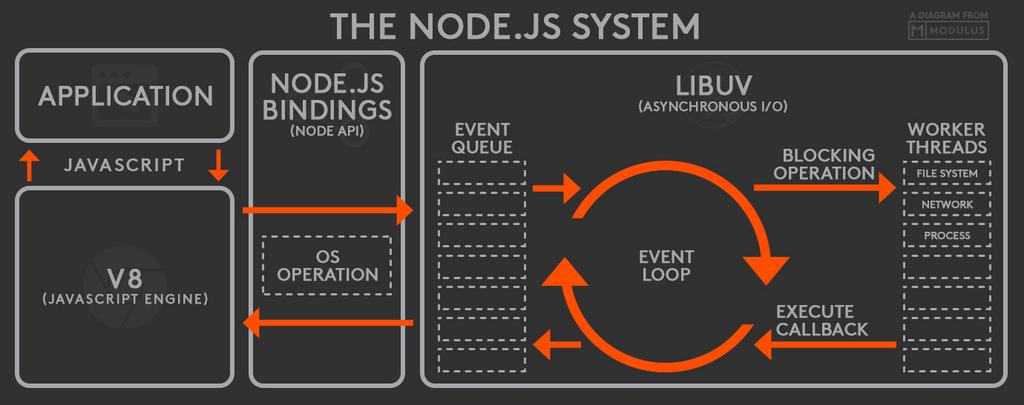
\includegraphics[width=.85\textwidth]{imagem/node-js-system-twitter-BusyRich.png}
    % Caption centralizada
    \captionsetup{justification=centering}
    \captionfont{\small{\textbf{\\Fonte: \cite{NodeSystem:2014}}}}	
    \label{fig:node-js-system-loop}
  \end{figure}
  
  A figura \ref{fig:node-js-system-loop} exibe uma síntese do sistema Node.JS. Primeiro a aplicação web requisita um evento 
  ao Node.Js instalado no servidor. Através da linguagem JavaScript V8 o Node.Js interage com sua \ac{API} e envia 
  a requisição para uma fila onde é processada pelo ciclo de eventos e tratada pelos módulos existentes no Node.js. 
  
  \citeonline{Pereira:2013} compara que a orientação a eventos do Node.Js se espelha na filosofia de orientação 
  a eventos utilizado nos navegadores; a diferença entre eles é que no Node.Js 
  não existe eventos de clique do mouse, teclas pressionadas do teclado (keyup) ou qualquer evento de componentes HTML. Mas operações
  de entrada e saída do servidor, assim como eventos de conexão ao banco de dados, abertura de arquivo e \textit{streaming}
  de dados.
  
  A principal diferença em sistemas baseados em eventos, é que o produtor do evento não espera pela ação a ser executada
  pelo servidor. \cite{Junior:2012}    

  Em complemento a esta abordagem o Node.Js inicia seu objetivo de criar aplicações de rede escaláveis, utilizando \textit{thread} única
  e o cilco de eventos para resolver os galargalos de altas conexões.

\section{Única thread e o cliclo de eventos}
\label{single-thread}

  Uma \textit{thread} pode ser conceituada como um conjunto de instruções executadas pelos processos do sistema operacional.
  Sendo que cada thread é um fluxo diferente de controle que pode executar estas instruções de forma independente, em exemplo,
  uma thread pode executar o GUI, enquanto uma segunda instrução faz alguns operações de entrada e saída, 
  enquanto um terceiro executa cálculos. \cite{Lewis:1995}
  
  Em Node.Js as conexões são recebidas em uma única \textit{thread} invocada pelo nó de servidor de processos \textit{node server process}.
  \citeonline{Abernethy:2011} cita que ao invés de criar novas \textit{threads}
  no sistema operacional para cada conexão e alocar a memória RAM que acompanha essas \textit{threads}, 
  cada conexão dispara um evento executado no processo do motor Node.Js.
  
  Isso ocorre porque ao ser invocado um nó de servidor de processos, ele roda apenas em 01 (uma) 
  \textit{thread} que suporta um alto número de conexões, isso é possível, pois há um \textit{loop} implícito que cobre o código, 
  essa repetição \textit{loop} é denominado de \textit{event loop} e tem como função esperar os eventos e repassá-los 
  ao manipulador de eventos. \cite{Tilkov:2010}
  
  \cite{Powers:2012} cita também o single \textit{thread} como um dos benefícios do ambiente do Node.Js 
  pois o aplicativo pode ser facilmente escalável uma vez que em um único segmento de execução não ha uma enorme 
  sobrecarga de requisições. Citando o exemplo de seu livro, ao criar uma aplicação em \ac{PHP} semelhante 
  à aplicação Node.Js o usuário veria a mesma página, mas ao visualzia os processos desta aplicação haverá uma 
  diferença.
  
  Este aplicativo \ac{PHP} no servidor web Apache, cada pedido que for solicitado irá abrir um 
  processo filho do Apache. Em servidores menos otimizados a capacidade de criar processos filhos
  restringe-se a par de centenas de processos filhos em paralelo. Se a por ventura a quantidade de solicitações
  for maior que capacidade de processos filhos do Apache, o cliente entrará numa fila e esperar por uma resposta.\cite{Powers:2012}

  Assim como \citeonline{Powers:2012}, \citeonline{Hughes:2012} afirma que o conceito de \textit{thread} única é importante para 
  toda a plataforma do Node.Js, porém é uma das críticas feitas ao Node.Js pela comunidade de desenvolvedores 
  que utilizando este conceito não é possivel realizar concorrência no nó de servidor de processos.
  
  \citeonline{Pereira:2013}, enfatiza que não é possível trabalhar com programação 
  concorrente em plataforma multi \textit{thread} nativamente com o ambiente Node.Js. Mas existem maneiras de implementar sistemas concorrentes, 
  como por exemplo, a utilização de clusters, o qual é um módulo nativo do ambiente Node.Js.
  
  Como a biblioteca  multi-node \citeonline{Zyp:2010}, é possivel compartilhar sockets nos servidores.
  Desta maneira o nó de servidor de processos pode ser instanciado em um ou mais processadores, oferencendo paralelismo, 
  atendendo e recebendo requisições nas mesma porta. Cabendo ao sistema operacional atuar como balanceador de carga.\cite{Oliveira:2012}
  
  Em conjunto com a \textit{thread} única o ambiente Node.Js possui o cilo de eventos sendo o agente responsável por escutar e 
  emitir eventos dentro do sistema. Onde o ciclo de eventos é uma repetição infinita que a cada interação verifica em sua 
  fila de eventos se um determinado evento foi emitido ou se existem novos eventos. Estes eventos só aparecem na 
  fila quando são emitidos durante as suas interações na aplicação; quando ocorre, é emitido um evento, então este evento 
  é executado e enviados para a fila de executados.\cite{Pereira:2013}
  
  \cite{Pereira:2013} diz que a programação orientada a eventos do Node.Js 
  foi inspirado pelos \textit{frameworks} Event Machine\footnote{http://rubyeventmachine.com/} do 
  Ruby\footnote{https://www.ruby-lang.org/en/} e Twisted\footnote{https://twistedmatrix.com/trac/} do 
  Python\footnote{https://www.python.org/}, porém o ciclo de eventos do Node.Js é mais perfomático pois seu mecanismo 
  é nativamente executado de forma não bloqueante sendo o diferencial em relação a outros ambientes de programação.
  
  \cite{Wilson:2013} enaltece os eventos do Node.Js, fornecido pelo JavaScript. Em outras linguagens de programação 
  os fluxos de trabalho são em \textit{threads} múltiplas e concorrentes, onde cada \textit{thread} gasta a maioria de seu tempo aguardando 
  operações bloqueadoras de entrada e saída, tais como: leitura ou escrita em disco, manipulação do banco de dados 
  acesso a informações pela rede. O que não ocorre com o Node.Js.
   
  Intuitivamente o ciclo de eventos é associado a vida cotidiana onde cada solicitação de evento necessita de um retorno.
  
  Possuindo a base de como o ciclo de eventos funciona, o desenvolvedor é capaz de usá-lo em toda sua potencialidade, 
  conseguindo vantagens e evitando armadilhas dessa abordagem.\cite{Hughes:2012}
  
  Aprofundando \cite{Pereira:2013} cita o módulo EventEmitter o responsável por emitir estes eventos e em 
  grande maioria das bibliotecas exitentes no Node.Js utiliza as funcionalidades de eventos deste módulo. 
  No processo de execução do evento pode-se programar qualquer lógica de programação através do 
  mecanismo de chamada de retorno. Tal chamada de retorno pode ser executado através de uma função de escuta, 
  semanticamente conhecida pelo on().
  
  Essa seção é bem descrita e exemplificada por \cite{Wilson:2013} em seu livro que nos mostra o uso e o 
  desenvolvimento de eventos.

  \citeonline{Oliveira:2012} e \citeonline{Abernethy:2011} relatam que através da arquitetura do Node.js, a aplicação poderá 
  suportar dezenas de milhares de conexões simultâneas. Pois os bloqueios ou impasses não são características da plataforma ao
  realizar processamento de entradas e saídas. O único gargalo de um servidor Node.Js passa-se a ser a capacidade de 
  tráfego da aplicação.
  
\section{JavaScript, Chamadas de retorno e \textit{callback's hell}}
\label{chamadas-de-retorno-e-callback-hell}

  O JavaScript V8 casou-se muito bem com a orientação a eventos, pois provê nativamente
  o modelo de eventos assíncronos em operações de entrada e saída, além de suporte à chamadas de retorno.\cite{Oliveira:2012}
  
  E através do alto desempenho do JavaScript Enginie V8, do Google, foi possível alterar o contexto da linguagem de programação
  amplamente utilizada em interfaces de sites nos navegadores e aplicá-la em servidores web formando o ambiente Node.Js.
  
  O V8 utiliza umas das técnicas recentes de compiladores que permite que o código escrito em linguagem de alto nível,
  tal como o JavaScript, execute de forma semelhante a linguagens de baixo nível como C. O Node.Js também aproveita
  do paradigma de orientação a eventos da linguagem e retira proveito da disso para compor sua arquitetura.

  Ao escrever códigos em Node.Js é necessário ter em mente que os metódos implementados em JavaScript trabalhe com uma 
  chamada de retorno de cada vez, para que o programa seja compreensível e também capaz de executar rapidamente várias 
  tarefas de forma eficiente.\cite{Hughes:2012}

  As chamadas de retorno, é uma função especial associada a um determinado evento que tende a ser executada quando o evento
  é atingido evitando assim a espera da execução de um processo.\citeonline{Wilson:2013} 
  
  Como exemplificado, um programa JavaScript assíncrono ao fazer uma requisição 
  a um banco de dados especifica o que deve ser feito com os resultados do banco de dados, ele não espera a 
  finalização da requisição e continua a processar outras atividades existes no programa. 
  Apenas quando o resultado da requisição é retornado do banco de dados, a codificação para manipular os estes dados 
  é executado. \cite[p. 2]{Junior:2012}
  
  No ambiente de desenvolvimento Node.Js é importante entender e saber trabalhar com as chamadas assíncronas para conseguir
  aproveitar a performance oferecida pelo JavaScript no Node.Js.\cite{Pereira:2013} em seu livro exemplifica em código
  as diferenças entre uma função síncrona e assíncrona em relação ao tempo em que são executadas. 
  
  Em resumo, este código é uma repetição de 5 interações e a cada iteração desta repetição é criado um arquivo texto. O primeiro
  exemplo utiliza o modelo síncrono existente no módulo (\textit{File System}) nativo do Node.Js (\textit{fs.writeFileSync}).
  
  \begin{figure}[H]
    % Alterar espaçamentos antes e depois do caption
    \setlength{\abovecaptionskip}{0pt}
    \setlength{\belowcaptionskip}{0pt}
    % Caption
    \caption[Tempo de resposta, metódo síncrono bloqueante]{Tempo de resposta, metódo síncrono bloqueante}
    \centering
    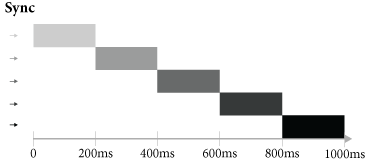
\includegraphics[width=.85\textwidth]{imagem/timeline-node-sync-caio-ribeiro.png}
    % Caption centralizada
    \captionsetup{justification=centering}
    \captionfont{\small{\textbf{\\Fonte: \cite{Pereira:2013}}}}	
    \label{fig:timeline-sync}
  \end{figure}
  
  A Figura \ref{fig:timeline-sync} exibe gráfico demonstrando que cada arquivo escrito
  gasta-se 200 milesegundos totalizando 1000 milesegundos para completar toda a tarefa.

  O segundo exemplo utiliza o mesmo módulo (\textit{File System}) implementando a função assíncrona. Esta função de acordo com
  a documentação \cite{ModuleSystemFs:2014} informa que obrigatoriamente precisa passar uma função de chamada de retorno como último
  parâmetro da função \textit{fs.writeFile}.
  

  Uma observação importante a ser feita descrita na documentação deste módulo e que 
  vale para todo o ambiente Node.Js e seus modulos é que os parâmetros passados para a chamada de retorno dependerá de 
  cada método, porém em regra   o primeiro argumento é sempre reservado para uma váriavel de erro ou exceção tratada no 
  escopo interno da chamada de retorno.
  Se a operação foi concluída com êxito, o primeiro argumento será nulo ou indefinido. \cite{ModuleSystemFs:2014}

  \begin{figure}[H]
    % Alterar espaçamentos antes e depois do caption
    \setlength{\abovecaptionskip}{0pt}
    \setlength{\belowcaptionskip}{0pt}
    % Caption
    \caption[Tempo de resposta, metódo assíncrono não-bloqueante]{Tempo de resposta, metódo assíncrono não-bloqueante}
    \centering
    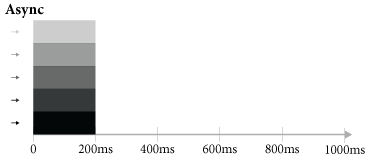
\includegraphics[width=.85\textwidth]{imagem/timeline-node-async-caio-ribeiro.png}
    % Caption centralizada
    \captionsetup{justification=centering}
    \captionfont{\small{\textbf{\\Fonte: \cite{Pereira:2013}}}}	
    \label{fig:timeline-async}
  \end{figure}

  A Figura \ref{fig:timeline-async} mostra o gráfico do tempo total de duração para escrever em 05 (cinco) arquivos. Essa 
  perfomance é dada a execução assíncrona que maximizou o processamento reduzindo o tempo total para 200 milesegundos.
  
  \cite{Pereira:2013} relata que o JavaScript possui boa performance trabalhando de forma assíncrona porém em certos 
  momentos do desenvolvimento, inevitavelmente será implementado diversas funções assíncronas encadeadas umas nas 
  outras através das chamadas de retorno criando o \textit{callbacks hell}.
  
  Em outro código \ref{leitura-arquivos-diretorio-node} implementado por \citeonline{Pereira:2013}, e referenciado no 
  Anexo \ref{primeiro-anexo} ha uma simples leitura de arquivos de um diretório qualquer sendo impresso o nome do arquivo 
  e seu tamanho em bytes. Este exemplo feito pelo autor demonstra que uma simples tarefa possui várias 
  chamadas de retorno encadeadas.
  
  Também questiona-se a organização do código escrito caso a solução do problema fosse mais complexa. Dando a entender que tal código
  seria um caos e de difícil manutenabilidade.
  
  Também é afirmado, que, a linguagem JavaScript por ser assíncrona resulta em ganhos de 
  performace, porém de perde-se o controle do que está sendo executado, e o acesso à variáveis devido às trocas de escopos
  neste emaranhado de chamadas de retorno.
  
  \citeonline{Pereira:2013} reafirma que as chamadas de retorno no Node.Js possuem como parâmetro uma variável de erro. Se existir
  este parâmetro, é recomendado que realize primeiramente o tratamento deste erro na execução da função
  impossibilitando a execução aleatória quando surgir tal erro.
  
  Uma das maneiras de se evitar o temido \textit{callback hell}, e dado que é, uma boa prática de codificação JavaScript é
  criar funções que expressem seu objetivo de forma isoladas, salvando os retornos em váriaveis e passando-as em outros
  chamadas de retorno como parâmetros. A organização do código pode ser visto no código \ref{leitura-arquivos-diretorio-node-callback-heaven} do
  Anexo \ref{primeiro-anexo}.\cite{Pereira:2013}
 
  Outra abordagem, utilizada pela empresa StrongLoop, é a utilização do módulo async \footnote{https://github.com/caolan/async},
  sendo o mais popular entre os desenvolvedores e também fica mais próximo do \textit{core} (núcleo) do Node.Js. Este módulo
  possui o metódo async.waterfall que provê um controle em série, em que os dados podem ser passados para a próxima função
  usando o parametro next. O metódo async.map executa o comando fs.stat (buscar status do arquivo) do Node.Js sobre uma matriz
  de caminhos, em paralelo. Em seguida retorna uma matriz com a ordem mantida dos resultados. Como dito pela empresa
  Strongloop, este módulo garante que somente uma chamada de retorno será retornada, propagação de erros e controle do 
  paralelismo automáticamente. 
  
  Outro módulo é apresentado pela empresa Strongloop é utilização de \textit{Promises} que fornece tratamento de erros
  e regalias de programação funcional. Para tal, é necessário utilizar o módulo Q \footnote{https://github.com/kriskowal/q}
  que através do metódo q.all executa todas as chamadas de status dos arquivos em paralelo e em seguida retorna uma matriz
  com a ordem dos dados mantidas. Ao contrário de exemplos anteriores, quaisquer exceção é lançada dentro da cadeia dos
  \textit{promises}. Somente depois tais exceções são capturadas e manipuladas.
  
  Por fim como descreve a \citeonline{Strongloop:2013} existe a abordagem utilizando \textit{generators} que estarão
  contemplatos e integrados oficialmente em versões posteriores à 0.11.2 do Node.Js. Os \textit{generators} podem ser definidos
  como co-rotinas leves para o JavaScript. Estes \textit{generators} permitem que uma função possa ser suspensa e retornada
  utilizando a palavra reservada yield. A empresa recomenda utilizar o módulo CO \footnote{https://github.com/visionmedia/co},
  mas nada impede a utilização de outros módulos. Ao utilizar o módulo CO é possível manipular erros (incluindo exceções levantadas)
  serão passadas para a função de chamada de retorno. Também é habilitado o uso de blocos \textit{try/catch} em torno das 
  declarações yield.
  
  Neste artigo \cite{Strongloop:2013} investigou-se três possibilidades de mitigar o problema dos \textit{callbacks hell}, com o 
  intuito de obtenção de controle do fluxo da aplicação. Um interesse maior surgiu pela a abordagem dos \textit{generators}
  apesar de não empregar em seus projetos. Independente de qual módulo e abordagem for utilizada ela reafirma que é recomendado
  utilizar a modularização em qualquer parte da aplicação e bibliotecas descritas (\textit{async,promises, generators}).
  
  Todo os código e comentários podem ser vistos no artigo da empresa. \cite{Strongloop:2013}
  

\section{O framework Express.Js}
\label{framework-express}

  \cite{Powers:2012} descreve que no geral um \textit{framework} ajuda na infraestrutura e que nos permite criar sites e aplicações
  com agilidade, fornecendo ao desenvolvedor um esqueleto capaz de oferecer um suporte no processo de desenvolvimento de
  software. Com os \textit{frameworks} foca-se na criação de funcionalidades da nossa aplicação ou site e 
  também fornece coesão ao código, o que nos beneficia com legibilidade e manutenabilidade.

  \cite{Pereira:2013} complementa que utilizar a API HTTP nativa do Node.Js pode ser um processo moroso e desgastante
  para o desenvolvedor. 
  Conforme surgem novas necessidades de implementação e novas funcionalidades serão acrescidas,
  os códigos se tornarão gigantescos aumentando a complexidade do projeto e dificultando futuras manutenções.
  
  Assim surge o \textit{framework} Express.Js para solucionar necessidades e agilizar no desenvolvimento.
  
  \citeonline{Powers:2012} compara que o \textit{Express.Js} é parecido com o \textit{framework} Sinatra porém bem mais \textit{RESTFUL}. 
  Pereira(2012) reafirma e complementa que o módulo \textit{Express.Js} foi inspirado pelo \textit{framework} Sinatra da 
  linguagem Ruby e que é bastante utilizado em aplicações web de grande escala.
  
  Suas características são descritas por \citeonline{Pereira:2013}:
  
  \begin{compactitem}
    \item[a)] \ac{MVR};   
    
    \item[b)] \ac{MVC};
    
    \item[c)] Roteamento de \ac{URL} com chamadas de retorno;
    
    \item[d)] Middleware;
    
    \item[e)] Interface \ac{REST};
    
    \item[f)] Suporte a File Uploads.
    
    \item[g)] Configuração baseada em variáveis de ambiente;
    
    \item[h)] Suporte a helpers dinâmicos;
    
    \item[i)] Integração com Templates Enginies;
    
    \item[j)] Integração com SQL e NoSQL;
    
  \end{compactitem}
  
  Ao criar um esqueleto utilizando o \textit{Express.js} é importante ter conhecimento do que cada
  arquivo ou diretório representa. \cite{Powers:2012, Hughes:2012} não apresentam um descritivo de cada arquivo 
  ou diretório e seu papel. Entretanto \cite{Pereira:2013, Wilson:2013} aprofundam mais neste assunto que podem ser vistos
  no apêndice \ref{apend:express-skel}.
  
  O arquivo de \textit{package.json}, de acordo com \citeonline{Wilson:2013} sempre é necessário ser criado 
  em seu projeto e que ele é responsável por fornecer detalhes sobre as condições de operação e configuração 
  esperadas por seu código. \cite{Wilson:2013} complementa que este arquivo ajuda a prevenir que alterações 
  futuras em módulos de terceiros quebrem a lógica da aplicação.

  No livro, \cite{Wilson:2013} exibe um exemplo do arquivo 
  \textit{package.json} o qual é utilizado para sincronizar a aplicação com dependências, sendo importante associar 
  a aplicação a uma versão especifica. 
  
  Para maiores detalhes sobre as notações semânticas utilizada pelo \ac{NPM} visite a documentação \cite{Semver:2013}.

\subsection{O servidor web com \textit{Express.Js}}
\label{servidor-web-express-js}

  
  De acordo com \cite{Wilson:2013} o interessante do Node.Js é que o código do 
  programa que se escreve para ele também é a implementação do servidor. 
  Seguindo este modelo tem-se a expectativa de que a aplicação funcione e se comporte de modo semelhante 
  ao ambiente de produção assim como no desenvolvimento, pois não existe nenhuma biblioteca, nenhum intermediário 
  ou \textit{daemon} que esteja no caminho.
  
  O arquivo app.js criado pelo \textit{Express.js} é em suma pequeno mas com grandes funcionalidades inclusas como 
  roteamento para solicitações \ac{HTTP} entrantes, motores de visões para renderizar marcações do HTML5
  e também download dos arquivos estáticos.